\documentclass{article}

\usepackage[utf8]{inputenc}
\usepackage{polski}
\usepackage{titlesec}
\usepackage{graphicx}
\usepackage[hidelinks]{hyperref}

\graphicspath{{images/}}

\title{Generator ruchu Google Analytics \\ Iteracja I architektura systemu}
\author{Bartłomiej Dalak \and Bartłomiej Karwowski \and Bartosz Gromek \and Tomasz Kanas}

\begin{document}
\maketitle

\section{Wstęp}

Dokument architektury systemu ma na celu przedstawienie wizji architektury. Opisana architektura może ulec zmianom w fazie implementacji.

\section{Opis elementów architektury}

\subsection{Aplikacja}

Aplikacją w naszym przypadku będzie skrypt ``generate\_ga\_traffic.py'', generujący ruch według podanych przez użytkownika wartości. Będzie on uruchamiany przez konsolę.

\subsubsection{Język}

Wykorzystany zostanie Python w wersji 3.6.

\subsubsection{Użyte biblioteki}

\begin{itemize}
\item \textbf{requests}: wysyłanie zapytań do GA i Measurement Protocol Validation Server
\item \textbf{pandas}: do obsługi pliku `browser.csv', w którym mamy rozkład przeglądarek na terenie Polski.
\end{itemize}

\subsection{send\_requests\_api}
API służące do komunkacji z GA, sprawdza dane od użytkownika, generuje potrzebne dane oraz je wysyła.

\subsubsection{Metody}
\begin{itemize}
\item \textbf{send(tracking\_id, url, visits\_no, time)}: sprawdza czy dane użytkownika mogą zostać wygenerowane, za pomocą funkcji \textbf{check\_data}. Jeśli dane przejdą tą weryfikację to przekazuje je do niżej opisanej funkcji \textbf{generate\_data}. Wpp. zwraca kod WRONG\_DATA. Po odebraniu wygenerowanych danych, próbuje przesłać je bezpośrednio do GA\@. Po otrzymaniu odpowiedzi zwraca jeden z 2 możliwych kodów {OK, CONNECTION PROBLEM}.

\item \textbf{check\_data(tracking\_id, url)}: metoda, która wyśle requesta do Measurement Protocol Validation Server za pomocą \textbf{requests.post("https://\\www.google-analytics.com/debug/collect",data={'tid': tracking\_id, 'dp': url, 'v': 1})} i jeśli otrzymany response w formacie JSON w polu ["hitParsingResult"][0]["valid"] zawiera wartość true to zwróci tuple(true, []), wpp. zwróci tuple(false, parameters), gdzie parameters to lista błędnych parametrów, które otrzymamy z pól ["hitParsingResult"][0]["parserMessege"] [i]["parameter"], gdzie i to indeks złego parametru.

\item \textbf{generate\_data(visits\_no)}: metoda wołana przez \textbf{send()}, generujące odpowiednie dane do wysłania. Po odebraniu informacji przekazanych przez użytkownika, do odpowiedniej ilości zapytań przypisuje dane przygotowane z wiarygodnym rozkładem. Informacje do tego potrzebne zostaną zczytane z pliku `browser.csv', który zostanie pobrany ze strony \href{http://gs.statcounter.com/browser-version-market-share/all/poland#monthly-201703-201803-bar}{GlobalStats StatCounter (dane\ dot.\ oprogramowania\ użytkowników\ witryny)}. Wykres użytkowania przeglądarek na terenie Polski.

\begin{center}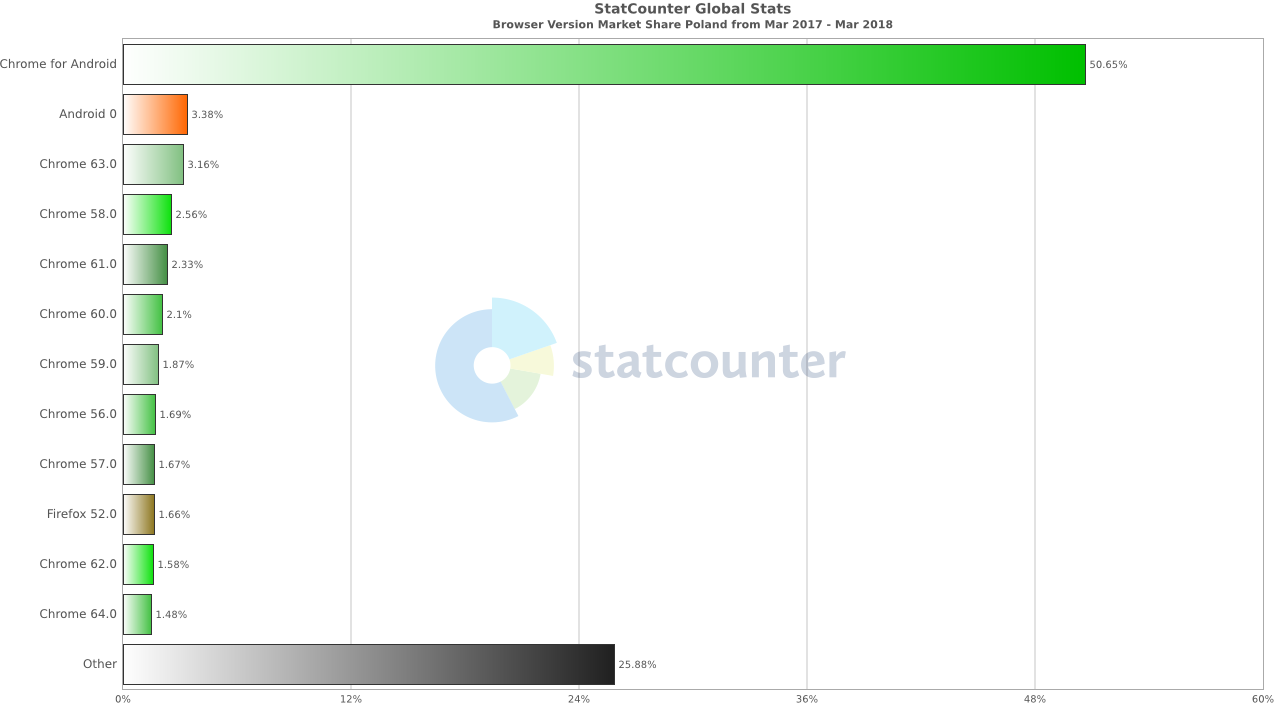
\includegraphics[scale=0.35]{chart}\end{center}
\end{itemize}

\section{Schemat działania}

\subsection{Generowanie i wysyłanie danych}
Dane otrzymane przez użytkownika zostaną przekazane do napisanego przez nas API: \textbf{send\_requests\_api}. API sprawdzi czy otrzymane dane od użytkownika są poprawne, wygeneruje zestaw wejść, które będą wysyłane do GA, a następnie za pomocą metody post z biblioteki \textbf{requests} wyśle je. 

\begin{center}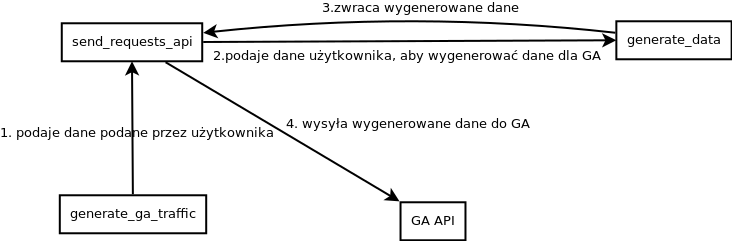
\includegraphics[scale=0.5]{connection_ga}\end{center}

\subsection{Wykrywanie braku połączenia z internetem}
Jeśli \textbf{send\_requests\_api} przez 10 min\. nie uda się wysłać żadnego requesta do GA API, w takim wypadku zostaje zatrzymane wysyłanie oraz zwrócony do generate\_ga\_traffic komunikat CONNECTION\_PROBLEM\@. Wtedy użytkownik zostaje o tym poinformowany i może wybrać jedną z trzech możliwości co chce robić dalej.

\end{document}
